%%%%%%%%%%%%%%%%%%%%%%%%%%%%%%%%%%%%%%%%%%%%%%%%%%%%%%%%%%%%%%%%%%
% FLAT — IEEE ICTAI 2026 short paper draft (<=5 pages, single file)
% Build:  cd paper && pdflatex root && bibtex root && pdflatex root && pdflatex root
% Figures: ./Figures/  
%%%%%%%%%%%%%%%%%%%%%%%%%%%%%%%%%%%%%%%%%%%%%%%%%%%%%%%%%%%%%%%%%%
\documentclass[conference]{IEEEtran}
\IEEEoverridecommandlockouts

\usepackage{cite}
\usepackage[T1]{fontenc}
\usepackage[final]{microtype}
\usepackage{indentfirst}
\usepackage{multirow}
\usepackage{amsmath,amssymb,amsfonts}
\usepackage{graphicx}
\graphicspath{{./Figures/}}
\usepackage{array}
\usepackage{tabularx}
\usepackage{booktabs}
\usepackage{makecell}
\usepackage[table]{xcolor}
\newcommand{\std}[1]{{\tiny\color{gray!90}$\pm$#1}}
\newcolumntype{L}{>{\raggedright\arraybackslash}X}
\newcolumntype{C}{>{\centering\arraybackslash}X}
\usepackage{url}
\usepackage{xurl}
\usepackage{float}
\usepackage[caption=false,font=footnotesize,labelfont=rm]{subfig}
\usepackage{tikz}
\usepackage{pgfplots}
\pgfplotsset{compat=1.18}
\usepackage{algorithm}
\usepackage{algpseudocode}
\newcommand{\ThanksPar}{\par}
\def\BibTeX{{\rm B\kern-.05em{\sc i\kern-.025em b}\kern-.08em
    T\kern-.1667em\lower.7ex\hbox{E}\kern-.125emX}}
\hyphenation{SUMO TraCI cal-i-bra-tion sur-ro-gate}
\pdfminorversion=4
\pdfobjcompresslevel=0

% Subfigure labels (Times). Fig. 1: fixed 16:9 box (stretch). Fig. 2/3: PDF, width-only.
\newcommand{\subcap}[1]{{\fontfamily{ptm}\selectfont #1}}
\newcommand{\panelw}{0.48\columnwidth}
\newcommand{\panelh}{\dimexpr0.48\columnwidth*9/16\relax}
\newcommand{\panelwfull}{\columnwidth}
\newcommand{\sceneimg}[1]{\includegraphics[width=\panelw,height=\panelh]{#1}}
\newcommand{\plotpanel}[1]{\includegraphics[width=\panelw,keepaspectratio]{#1}}
\newcommand{\plotpanelfull}[1]{\includegraphics[width=\panelwfull,keepaspectratio]{#1}}

\title{FLAT: Smoothing the Rugged Landscape for Learnable, Sample-Efficient Traffic Calibration}

\author{\IEEEauthorblockN{Haopeng Deng}
\IEEEauthorblockA{\textit{School of Future Transportation} \\
\textit{Guangzhou Maritime University}\\
Guangzhou 510725, China \\
qianyhp@gmail.com}
\and
\IEEEauthorblockN{Shuo He$^{*}$}
\IEEEauthorblockA{\textit{Department of Civil and Environmental Engineering} \\
\textit{Imperial College London}\\
London SW7 2AZ, United Kingdom \\
sh4124@ic.ac.uk}
\and
\IEEEauthorblockN{Dayuan Wang}
\IEEEauthorblockA{\textit{Department of Biostatistics} \\
\textit{University of Florida}\\
Gainesville, FL 32601, USA \\
dayuan.wang@ufl.edu}}

\begin{document}
\maketitle

\begin{abstract}
Calibrating microscopic traffic simulators is an expensive black-box problem with a rugged landscape: tuning car-following and lane-changing parameters requires a full SUMO--TraCI run, affording only a tight budget per scene. Matching raw trajectories yields a rugged, scene-dependent objective that sparse surrogates cannot learn, reducing sequential acquisition to near-random probing. We present FLAT to couple two decisions: \emph{what} to optimize and \emph{where} to sample next. An eight-dimensional behavioral fingerprint smooths the parameter--error landscape, making a surrogate learnable from a few dozen samples; annealed lower-confidence-bound (LCB) acquisition then spends each remaining run where it most reduces error. The surrogate, a random forest or a multi-layer-perceptron (MLP) ensemble, is interchangeable. Across six heterogeneous SIND/UTE scenes and five seeds, FLAT significantly outperforms four optimizer families (SPSA, GA, CMA-ES, TPE) under matched budgets (Wilcoxon $p<0.05$), cutting the simulation cost of reaching equivalent quality by up to $4\times$. Ablations trace the gain to objective geometry and sequential allocation rather than surrogate capacity.
\end{abstract}

\begin{IEEEkeywords}
Surrogate-assisted optimization; traffic simulation calibration; behavioral fingerprint; sample-efficient learning.
\end{IEEEkeywords}

%======================================================================
\section{Introduction}
\label{sec:introduction}
% See docs/PAPER_OUTLINE_ICTAI.md §II for full narrative

Operational decisions in urban traffic increasingly rely on real-time digital twins~\cite{ref_dt}. Their credibility, however, rests on a microscopic simulator such as SUMO~\cite{ref_sumo} reproducing \emph{how} vehicles actually move, not merely average flow. That fidelity is only as good as the car-following~\cite{ref_krauss} and lane-changing~\cite{ref_lc2013} parameters governing each vehicle, which must be calibrated per location from observed trajectories. Because each candidate vector is scored only by rerunning the full network, calibration is an expensive, stochastic, black-box optimization problem in which only about $10^2$ runs are affordable per scene.

Two schools address it. The first searches the raw objective directly with general-purpose optimizers---genetic algorithms (GA)~\cite{ref_ga}, simultaneous perturbation stochastic approximation (SPSA)~\cite{ref_spsa}, and the covariance matrix adaptation evolution strategy (CMA-ES)~\cite{ref_cmaes}---which are derivative-free but sample-hungry: in ten dimensions an evolution strategy completes only a handful of generations within a hundred runs, and none remembers where expensive evaluations have already probed. The second school is surrogate-assisted, or Bayesian, optimization, which fits a cheap model of the response surface to decide where to evaluate next; the idea was formalized by Jones~\textit{et~al.}~\cite{ref_surrogate2} and is now standard for costly simulators~\cite{ref_surrogate1}, using tree-structured Parzen estimation (TPE)~\cite{ref_tpe,ref_optuna}, Gaussian-process~\cite{ref_pracbo}, or random-forest (RF)~\cite{ref_rf} surrogates, with recent transport work calibrating large traffic models this way~\cite{ref_bocal,ref_aical,ref_bo4mob}. Yet both schools take the objective and the budget allocation as given, even though no single optimizer consistently outperforms others across diverse calibration setups: parameter sets, goodness-of-fit measures, and case studies all shift which method wins~\cite{ref_calibration}.

That instability reflects a shared assumption: surrogate methods presuppose an objective that is learnable from few samples, yet in microscopic calibration the natural target, per-vehicle trajectory matching, is high-dimensional, rugged, and scene-dependent, preventing reliable surrogate learning and reducing acquisition to near-random probing. The literature keeps refining the optimizer or the surrogate family while leaving two upstream choices implicit: the \emph{geometry of the objective} a surrogate must learn, and \emph{how a fixed budget is split} between exploration and exploitation. The gap is therefore not accuracy but mechanism: without a learnable objective, sample-efficient acquisition has nothing to exploit, and performance rankings reverse across scenes rather than methods.

We instantiate this as \textbf{FLAT} (Fingerprint-guided Learnable Acquisition for Traffic Calibration), which makes both choices explicit. For the objective, it replaces trajectory matching with a compact \emph{behavioral fingerprint} that smooths the parameter-to-error landscape, enabling reliable surrogate learning from a few dozen runs. For the budget, an uncertainty-aware acquisition policy allocates the remaining simulation sequentially, annealing exploration into exploitation as the budget depletes. The framework is surrogate-agnostic, which lets us test whether efficiency comes from model capacity or from how the problem is posed; our ablations point to the latter.

\begin{figure*}[t]
  \centering
  \vspace{-4pt}
  \includegraphics[width=\textwidth,keepaspectratio]{{architecture of the FLAT}}
  \caption{FLAT overview. Parameters $\theta$ (Krauss/LC2013) are evaluated in SUMO--TraCI; observed and simulated trajectories are compressed into behavioral fingerprints and scored by weighted relative error $J_b(\theta)$. A pluggable surrogate (RF or MLP) returns $(\mu,\sigma)$ for sequential LCB acquisition.}
  \label{fig:arch}
  \vspace{-4pt}
\end{figure*}

\textbf{Contributions.}
\begin{enumerate}
  \item We propose FLAT, a surrogate-acquisition framework that converts the rugged objective into a learnable surface via behavioral representation reshaping, enabling sample-efficient calibration within ${\sim}10^2$ evaluations per scene.
  \item We establish a consistent, significant advantage over four mechanistically diverse optimizer families across six real-world scenes, with competitors requiring up to $4\times$ more simulations to reach equivalent quality.
  \item We trace the gain to objective geometry and sequential allocation, not surrogate capacity, establishing objective learnability as a prerequisite for surrogate guidance; code and cache are openly released for reproducibility.
\end{enumerate}

%======================================================================
\section{Problem Formulation}
\label{sec:problem}

Microscopic calibration tunes a ten-dimensional parameter vector $\theta\in\mathbb{R}^{10}$---six car-following parameters of the Krauss model~\cite{ref_krauss} and four lane-changing parameters of the LC2013 model~\cite{ref_lc2013}---written into SUMO~\cite{ref_sumo} at runtime via TraCI, the traffic control interface. Each candidate $\theta$ is scored by running a full simulation and comparing the resulting driving behavior against real trajectories, so every evaluation costs one complete SUMO run. Under an affordable budget of $B$ we seek
\begin{equation}
  \theta^\star = \arg\min_{\theta\in\Theta}\, J(\theta) \quad\text{within } B \text{ evaluations of } J,
  \label{eq:problem}
\end{equation}
where $\Theta\subset\mathbb{R}^{10}$ collects the per-scene parameter bounds and $J(\theta)$ quantifies some behavioral discrepancy between simulated and observed driving. The map $\theta\mapsto J(\theta)$ has no closed form and is costly to query---an \emph{expensive black-box optimization} problem in which sample efficiency is the central concern.

\section{FLAT Method}
\label{sec:method}

Fig.~\ref{fig:arch} overviews the framework. FLAT follows one principle: \emph{spend each simulation where it carries the most information}. Two coupled decisions realize it---\emph{what} to optimize and \emph{where} to sample next---via a behavioral-fingerprint objective (\S\ref{sec:objective}) and a sequential acquisition loop with a pluggable surrogate (\S\ref{sec:acq}--\S\ref{sec:surrogate}). Algorithm~\ref{alg:bfsac} details the steps.

\begin{algorithm}[h]
  \caption{FLAT calibration under simulation budget $B$.}
  \label{alg:bfsac}
  {\small
  \begin{algorithmic}[1]
    \Require Scene config; real fingerprint $\mathbf{f}^{\mathrm{real}}$; bounds; $N_{\mathrm{init}}$; schedule $\kappa_t$
    \Ensure Calibrated $\theta^\star$ and history $\{(\theta_i, J_b(\theta_i))\}_{i=1}^{B}$
    \State Draw $\{\theta_i\}_{i=1}^{N_{\mathrm{init}}}$ by Latin-hypercube sampling (LHS); evaluate $J_b$ in SUMO \Comment{Phase A}
    \For{$t = N_{\mathrm{init}}+1,\ldots,B$} \Comment{Phase B}
      \State Fit surrogate $(\mu,\sigma)$ on $\{(\theta_i,J_b(\theta_i))\}_{i<t}$
      \State $\theta_{\mathrm{best}} \leftarrow \arg\min_{i<t} J_b(\theta_i)$; sample trust region around $\theta_{\mathrm{best}}$ + global candidates; drop near-duplicates
      \State $\theta_t \leftarrow \arg\min_\theta\, \mu(\theta)-\kappa_t\,\sigma(\theta)$
      \State Evaluate $J_b(\theta_t)$ in SUMO; append
    \EndFor
    \State \Return $\theta^\star=\arg\min_i J_b(\theta_i)$
  \end{algorithmic}
  }
\end{algorithm}

\subsection{Behavioral Fingerprint Objective}
\label{sec:objective}
Matching raw per-vehicle trajectories yields an objective that is rugged, high-variance, and scene-dependent; under ${\sim}10^2$ samples no lightweight surrogate can learn it, so the search degenerates into near-random probing. We instead compress each trajectory set into an eight-dimensional \emph{behavioral fingerprint} $\mathbf{f}=(v_{\mathrm{mean}},\,v_{15},\,v_{85},\,\bar{a}^{+},\,\bar{a}^{-},\,a_{5},\,a_{95},\,s_{\mathrm{stop}})$---mean speed, its $15$th/$85$th percentiles, mean positive and negative acceleration, the $5$th/$95$th acceleration percentiles, and the stop fraction---and minimize the weighted, clipped relative error between simulated and real fingerprints:
\begin{equation}
  J_b(\theta) = \sum_{k=1}^{8} w_k \,\min\!\left(\frac{|f_k^{\mathrm{sim}}(\theta)-f_k^{\mathrm{real}}|}{\max(|f_k^{\mathrm{real}}|,\epsilon)},\; 3\right).
  \label{eq:jb}
\end{equation}
The weights $w_k$ and the per-parameter bounds encode light traffic-domain priors---e.g.\ intersections emphasize the stop fraction, freeways the speed spread. The smoothing is directly visible in Fig.~\ref{fig:landscape}: over 400 SUMO runs on the XAM expressway, the raw per-second speed RMSE surface is highly irregular, whereas $J_b$ yields a structurally smoother landscape---the precondition for the surrogate to guide sequential acquisition.
\begin{figure}[h]
  \centering
  \vspace{-4pt}
  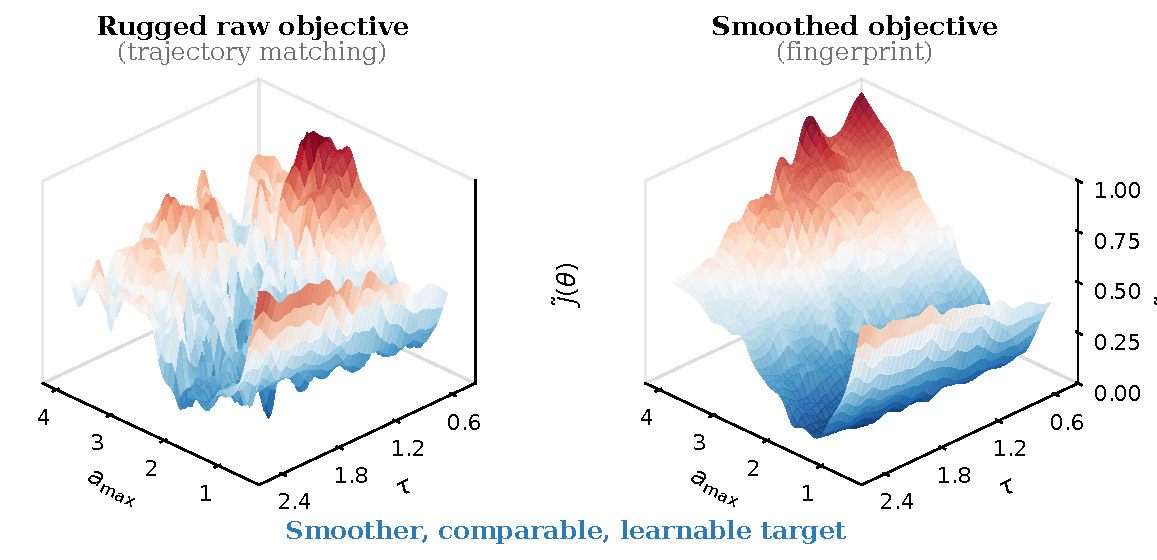
\includegraphics[width=\columnwidth]{landscape_dual_XAM-N6.pdf}
  \caption{Objective landscape in the $(a_{\max},\tau)$ plane (400 SUMO
    evaluations, XAM expressway); both surfaces normalized to $[0,1]$
    for shape comparison.
    \emph{Left:} raw per-second speed RMSE. \emph{Right:} fingerprint $J_b$.}
  \label{fig:landscape}
  \vspace{-4pt}
\end{figure}

\subsection{Sequential Acquisition}
\label{sec:acq}
A fixed budget $B{=}100$ is split into an exploratory Phase~A and a refinement Phase~B. Phase~A draws $N_{\mathrm{init}}{=}40$ Latin-hypercube (LHS)~\cite{ref_lhs} samples over $\theta$ for coverage and evaluates each in SUMO. Phase~B then spends the remaining $B-N_{\mathrm{init}}$ simulations sequentially: at each step it (i) fits a surrogate that returns a predictive mean $\mu(\theta)$ and uncertainty $\sigma(\theta)$ on observed $(\theta,J_b)$ pairs, (ii) draws candidates from a trust region around the current incumbent ($\pm18\%$ of each parameter's span) together with a global pool, (iii) selects the candidate that minimizes the lower confidence bound (LCB)
\begin{equation}
  \mathrm{LCB}(\theta) = \mu(\theta) - \kappa\,\sigma(\theta),
  \label{eq:lcb}
\end{equation}
after discarding points too close to evaluated ones, and (iv) evaluates it in SUMO and appends the result. The uncertainty term $\sigma$ lets the acquisition explore where the surrogate is unsure and exploit where it is confident. Over the $B-N_{\mathrm{init}}$ sequential steps $t$ we anneal $\kappa$ linearly,
\begin{equation}
  \kappa_t = \kappa_0 + (\kappa_T-\kappa_0)\,\frac{t}{B-N_{\mathrm{init}}-1}, \quad \kappa_0{=}2.0,\ \kappa_T{=}0.5,
  \label{eq:kappa}
\end{equation}
shifting the balance from exploration to exploitation as the budget depletes. On the same XAM slice (Fig.~\ref{fig:lcb}), Phase-B trials concentrate in the low-$J_b$ valley after Phase-A coverage. Pure space-filling spends the same budget without this feedback, which the ablation in \S\ref{sec:gain} shows to be markedly worse.
\begin{figure}[h]
  \centering
  \vspace{-4pt}
  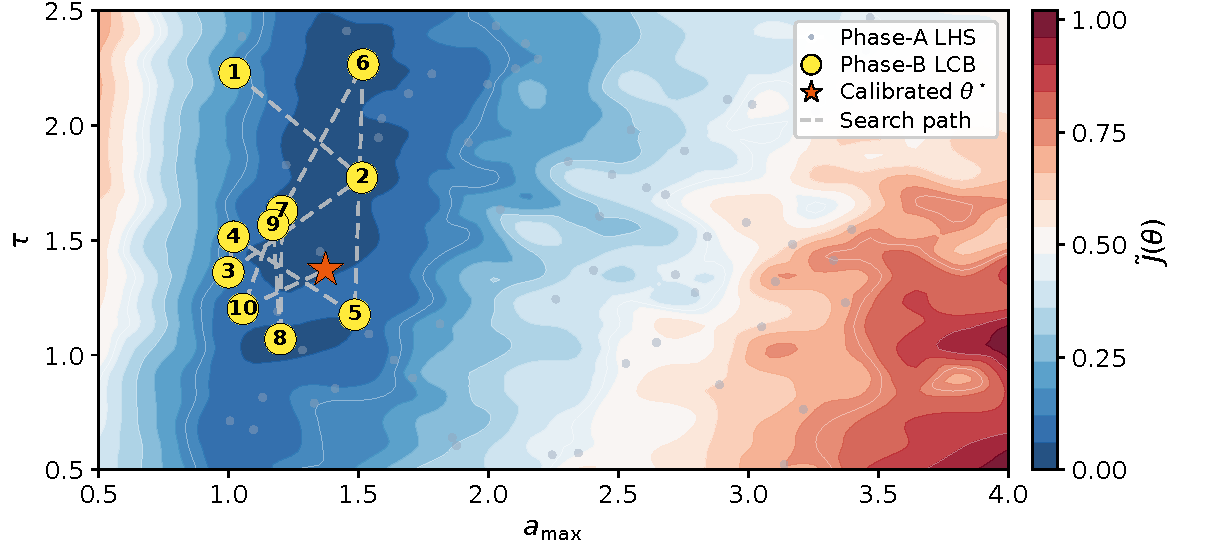
\includegraphics[width=\columnwidth]{lcb_contour.pdf}
  \caption{Sequential acquisition in the $(a_{\max},\tau)$ plane
    (XAM expressway, $B{=}100$, $N_{\mathrm{init}}{=}40$);
    $\tilde{J}(\theta)$ normalized to $[0,1]$.}
  \label{fig:lcb}
  \vspace{-4pt}
\end{figure}

\subsection{Pluggable ML Surrogates}
\label{sec:surrogate}
The acquisition loop is surrogate-agnostic: any learner that returns a predictive mean $\mu(\theta)$ and uncertainty $\sigma(\theta)$ can serve, leaving the surrogate freely exchangeable. We specifically instantiate two representative ML regression models to test whether performance depends on surrogate capacity. Concretely, for an $M$-member ensemble on $\mathcal{D}{=}\{(\theta_i,J_b(\theta_i))\}$,
\begin{equation}
  \mu(\theta)=\frac{1}{M}\sum_{m=1}^{M}h_m(\theta),\quad
  \sigma(\theta)=\sqrt{\tfrac{1}{M}\sum_{m=1}^{M}\!\bigl(h_m(\theta)-\mu(\theta)\bigr)^{2}},
  \label{eq:ensemble}
\end{equation}
feeding directly into \eqref{eq:lcb}. The lightweight default is a random forest~\cite{ref_rf} of $M{=}500$ bootstrap-bagged regression trees (no input normalization; $\sigma$ from inter-tree spread); the higher-capacity alternative is an MLP ensemble~\cite{ref_ensemble} of $M{=}10$ two-layer $(64,64)$ networks, each trained independently on a bootstrap resample of $\mathcal{D}$ with standardized inputs ($\sigma$ scaled by $1.2$ to prevent overconfident acquisition). Both plug into the identical LCB loop, with \S\ref{sec:gain} verifying whether performance depends on surrogate capacity.

%======================================================================
\section{Experiments}
\label{sec:experiments}

\subsection{Setup}
We evaluate on six heterogeneous real-world scenes reconstructed as SUMO networks from SIND~\cite{ref_sind} and UTE~\cite{ref_ute} aerial trajectories (Fig.~\ref{fig:scenes}): three signalized intersections (Tianjin, Changchun, Xi'an) spanning a low-to-high saturation range, and three urban-expressway segments (YTDJ, RML, XAM) covering merge and weaving bottlenecks.
\begin{figure}[h]
  \vspace{-4pt}
  \centering
  \subfloat[\subcap{Tianjin}]{\sceneimg{scene_tianjin.jpg}\label{fig:scene_tj}}
  \hfill
  \subfloat[\subcap{YTDJ}]{\sceneimg{scene_ytdj.png}\label{fig:scene_ytdj}}
  \\
  \subfloat[\subcap{Changchun}]{\sceneimg{scene_changchun.jpg}\label{fig:scene_cc}}
  \hfill
  \subfloat[\subcap{RML}]{\sceneimg{scene_rml.png}\label{fig:scene_rml}}
  \\
  \subfloat[\subcap{Xi'an}]{\sceneimg{scene_xian.jpg}\label{fig:scene_xa}}
  \hfill
  \subfloat[\subcap{XAM}]{\sceneimg{scene_xam.png}\label{fig:scene_xam}}
  \caption{Six heterogeneous evaluation scenes: three signalized intersections (left, SIND) and three urban-expressway segments (right, UTE).}
  \label{fig:scenes}
  \vspace{-4pt}
\end{figure}
\textbf{Protocol.} Every method receives the same budget $B{=}100$, the same objective $J_b$, the same per-scene bounds, and the seed set $\{42,101,202,303,404\}$; we report the best $J_b$ achieved within the budget.
\textbf{Baselines.} We compare FLAT-RF and FLAT-MLP ($N_{\mathrm{init}}{=}40$) against four optimizer families: SPSA~\cite{ref_spsa} (gradient estimation), GA (population search), CMA-ES~\cite{ref_cmaes} (evolution strategy), and TPE~\cite{ref_tpe,ref_optuna} (density-estimation Bayesian optimizer).
\textbf{Significance.} We run one-sided paired Wilcoxon signed-rank tests~\cite{ref_wilcoxon} over the $6\times5=30$ scene$\times$seed points.

\subsection{Best Under Equal Budget}
\label{sec:results}
Under matched budget, FLAT attains the lowest mean error among all methods (Table~\ref{tab:main}): RF and MLP reach $J_b=0.241$ and $0.240$, ahead of TPE ($+6.7\%$), GA ($+14.7\%$), CMA-ES ($+16.3\%$), and SPSA ($+59.3\%$). Because these baselines cover four different optimization mechanisms, the consistent margin indicates that the advantage is intrinsic to the method rather than a coincidental fit to one algorithm family. The paired Wilcoxon tests (Table~\ref{tab:main}) sharpen this: FLAT-RF wins $20$--$28/30$ pairs against all four baselines (all $p<0.05$); FLAT-MLP is equally significant across all four baselines (lowest $p{=}0.044$, $16/30$ vs.\ TPE), so the lead holds across most (scene, seed) pairs and is not driven by a single scene. Fig.~\ref{fig:panel} shows FLAT keeps the narrowest seed band throughout the budget ($\pm0.006$--$0.009$ vs.\ $\pm0.043$ for SPSA), indicating that the advantage is consistent across seeds rather than driven by lucky initializations. The ranking reflects each family's mechanism: TPE's density-ratio model $p(\theta\mid J_b)$ exploits parameter coupling less directly than our regression surrogate with LCB; CMA-ES cannot sustain more than ${\sim}10$ generations in ten dimensions within the budget; and SPSA's gradient estimates destabilize on rugged scenes (e.g.\ Changchun). FLAT descends steadily past the LHS-to-sequential transition where all four stall. Fig.~\ref{fig:speeddist} corroborates this at the speed level, with mean distributional similarity $\bar{\rho}{=}0.77$.

\begin{table}[h]
  \caption{Six-scene mean $J_b$ at budget $100$, five seeds; values shown as mean with seed std. Won/30 and $p$: one-sided paired Wilcoxon, $H_1{:}$ FLAT-RF $<$ baseline, $n{=}30$.}
  \label{tab:main}
  \centering\setlength\tabcolsep{4pt}\footnotesize\renewcommand{\arraystretch}{1.15}
  \begin{tabularx}{\columnwidth}{@{}l C C C C C@{}}
    \toprule
    & & \multicolumn{2}{c}{$\Delta\%$ vs.} & & \\
    \cmidrule(lr){3-4}
    Method & Mean $J_b\downarrow$ & RF & MLP & Won/30 & $p$ \\
    \midrule
    FLAT-RF  & \textbf{0.241}\,\std{0.009} & ---    & $+0.1$  & ---    & ---    \\
    FLAT-MLP & 0.240\,\std{0.006}          & $-0.1$ & ---     & ---    & ---    \\
    TPE      & 0.257\,\std{0.010}          & $+6.7$  & $+6.9$  & 20/30  & 0.009  \\
    GA       & 0.276\,\std{0.013}          & $+14.7$ & $+14.8$ & 24/30  & ${<}0.001$ \\
    CMA-ES   & 0.280\,\std{0.023}          & $+16.3$ & $+16.4$ & 24/30  & ${<}0.001$ \\
    SPSA     & 0.383\,\std{0.043}          & $+59.3$ & $+59.5$ & 28/30  & ${<}0.001$ \\
    \bottomrule
  \end{tabularx}
\end{table}

\begin{figure}[h]
  \centering
  \plotpanelfull{method_comparison_convergence.pdf}
  \caption{Running best-so-far $J_b$ averaged over six scenes and five seeds ($B{=}100$). Shaded bands: $\pm1$\,std across seeds; dotted line: budget cap.}
  \label{fig:panel}
\end{figure}

\begin{figure}[t]
  \centering
  \plotpanelfull{speed_distribution_violin.pdf}
  \caption{Observed vs.\ simulated speed distributions under FLAT-RF calibration. Per-scene similarity $\rho{=}1{-}D_{\mathrm{KS}}$; stars and ticks mark $v_{\mathrm{mean}}$, $v_{15}$, and $v_{85}$.}
  \label{fig:speeddist}
\end{figure}

\subsection{Cheapest to Equal Quality}
\label{sec:efficiency}
To put the advantage in concrete cost terms, we extend each baseline's budget to $500$ and record, for each of 30 scene$\times$seed pairs, the first simulation at which its running-best $J_b$ matches FLAT-RF's (or FLAT-MLP's) per-scene mean at $B{=}100$ (Table~\ref{tab:efficiency}). Even TPE, the strongest competitor, requires $1.67\times$ the budget; CMA-ES and GA need $2.9\times$ and $3.6\times$; SPSA reaches the threshold in only $9/30$ pairs within the cap. FLAT's edge is therefore not a marginal numerical improvement but a concrete reduction in simulation cost.

\begin{table}[h]
  \caption{Simulations needed to match FLAT@100, mean\,$\pm$\,std over $30$ scene\,$\times$\,seed pairs, budget capped at $500$. Reach: pairs reaching the quality threshold within cap, vs.\ FLAT-RF.}
  \label{tab:efficiency}
  \centering\footnotesize\renewcommand{\arraystretch}{1.15}
  \begin{tabularx}{\columnwidth}{@{}l C C C C C@{}}
    \toprule
    & \multicolumn{2}{c}{vs.\ FLAT-RF} & \multicolumn{2}{c}{vs.\ FLAT-MLP} & \\
    \cmidrule(lr){2-3}\cmidrule(lr){4-5}
    Baseline & Sims$\downarrow$ & Ratio & Sims$\downarrow$ & Ratio & Reach$\uparrow$ \\
    \midrule
    TPE    & 167\,\std{139} & 1.67$\times$ & 147\,\std{140} & 1.47$\times$ & 28/30 \\
    CMA-ES & 288\,\std{148} & 2.88$\times$ & 276\,\std{108} & 2.76$\times$ & 25/30 \\
    GA     & 360\,\std{165} & 3.60$\times$ & 305\,\std{170} & 3.05$\times$ & 15/30 \\
    SPSA   & 409\,\std{159} & 4.09$\times$ & 424\,\std{154} & 4.24$\times$ &  9/30 \\
    \bottomrule
  \end{tabularx}
\end{table}

\subsection{Sources of Performance Gain}
\label{sec:gain}
We attribute the advantage to two design choices and verify each. \textbf{Sequential acquisition is causal.} The $N_{\mathrm{init}}$ sweep (Fig.~\ref{fig:ninit}) fixes the budget at $100$ and varies how much of it is space-filling; pure LHS ($N_{\mathrm{init}}{=}100$, no sequential step) is the worst or near-worst configuration on every scene---for instance Changchun rises from $0.168$ to $0.236$ and Tianjin from $0.146$ to $0.182$---so the improvement stems from LCB-guided refinement, not from a richer initial design, with the optimum near $N_{\mathrm{init}}{=}20$--$40$. \textbf{The gain is structural, not model capacity.} The two surrogates track each other and coincide on average (Fig.~\ref{fig:percalib}). On easy-to-fit scenes---XAM, Tianjin, and Changchun, where RF achieves $R^2\!\geq\!0.97$---the two surrogates converge within $0.02$ of each other and RF is often marginally lower; on harder scenes (Xi'an, YTDJ, RML), MLP's higher capacity reduces error more visibly, most markedly on RML ($J_b$: $0.434\!\to\!0.408$, surrogate $R^2$ from $0.976$ to $0.997$). Neither surrogate decisively dominates the other, confirming that surrogate capacity is not the primary lever. \textbf{The fingerprint makes the objective learnable.} The per-scene $R^2$ annotations in Fig.~\ref{fig:percalib} show the surrogate already reaches $R^2\ge0.94$ from only the $40$ LHS samples---confirming that the fingerprint delivers the learnability that makes sequential acquisition effective.
\begin{figure}[t]
  \centering
  \subfloat[\subcap{Tianjin}]{\plotpanel{calib_conv_tianjin.pdf}\label{fig:calib_tj}}
  \hfill
  \subfloat[\subcap{YTDJ}]{\plotpanel{calib_conv_ytdj.pdf}\label{fig:calib_ytdj}}
  \\
  \subfloat[\subcap{Changchun}]{\plotpanel{calib_conv_changchun.pdf}\label{fig:calib_cc}}
  \hfill
  \subfloat[\subcap{RML}]{\plotpanel{calib_conv_rml.pdf}\label{fig:calib_rml}}
  \\
  \subfloat[\subcap{Xi'an}]{\plotpanel{calib_conv_xian.pdf}\label{fig:calib_xa}}
  \hfill
  \subfloat[\subcap{XAM}]{\plotpanel{calib_conv_xam.pdf}\label{fig:calib_xam}}
  \caption{Per-scene best-so-far $J_b$ convergence for both surrogates, five-seed mean $\pm1$\,std. Dashed line at $N_{\mathrm{init}}{=}40$ marks the LHS-to-sequential transition.}
  \label{fig:percalib}
  \vspace{-8pt}
\end{figure}

\begin{figure}[t]
  \centering
  \subfloat[\subcap{Tianjin}]{\plotpanel{n_init_tianjin.pdf}\label{fig:ninit_tj}}
  \hfill
  \subfloat[\subcap{YTDJ}]{\plotpanel{n_init_ytdj.pdf}\label{fig:ninit_ytdj}}
  \\
  \subfloat[\subcap{Changchun}]{\plotpanel{n_init_changchun.pdf}\label{fig:ninit_cc}}
  \hfill
  \subfloat[\subcap{RML}]{\plotpanel{n_init_rml.pdf}\label{fig:ninit_rml}}
  \\
  \subfloat[\subcap{Xi'an}]{\plotpanel{n_init_xian.pdf}\label{fig:ninit_xa}}
  \hfill
  \subfloat[\subcap{XAM}]{\plotpanel{n_init_xam.pdf}\label{fig:ninit_xam}}
  \caption{$N_{\mathrm{init}}$ ablation: final $J_b$ vs.\ warm-up size at fixed budget $100$, five-seed mean $\pm1$\,std. $N_{\mathrm{init}}{=}100$ reduces to pure LHS.}
  \label{fig:ninit}
  \vspace{-8pt}
\end{figure}

\subsection{Operating Range}
\label{sec:limits}
The advantage concentrates on moderately rugged scenes (e.g.\ YTDJ, RML, Changchun), where ``looking before leaping'' matters and surrogate guidance avoids the wasted or unstable evaluations of the baselines. Two limiting regimes bound the applicability. On the easy XAM ($J_b\approx0.044$) the optimum is broad and all methods nearly tie. On Xi'an, Fig.~\ref{fig:speeddist} shows the weakest distributional match at $\rho{=}0.53$, yet all six methods cluster near $J_b\approx0.43$ with a spread below $0.02$---here the residual error is an irreducible floor set by the mismatch between the fingerprint and the parameter space, not by optimizer weakness. These regimes delineate the operating range in which sample-efficient surrogate calibration is worthwhile.

%======================================================================
\section{Conclusion}
\label{sec:conclusion}

We presented FLAT, a framework that addresses the root cause of poor sample efficiency in surrogate-assisted traffic calibration: raw trajectory objectives are too rugged to be learned from few samples, leaving acquisition without a reliable signal. A behavioral fingerprint smooths the parameter-to-error landscape so that a sample surrogate can fit it from a few dozen samples, and annealed LCB acquisition then concentrates the remaining budget where it most reduces error. Across six heterogeneous scenes and four optimizer families, FLAT is consistently best under matched budgets; even with unlimited budgets, competitors need $1.7\times$--$4\times$ more simulations to match FLAT's $100$-run quality. Ablations confirm that the gain traces to objective geometry and sequential allocation rather than surrogate capacity. The finding suggests that objective geometry is the bottleneck in sample-limited black-box optimization, not surrogate capacity or acquisition design.

Future work will extend this insight by learning low-dimensional, surrogate-learnable behavioral objectives with self-supervised trajectory encoders, optionally pretrained on large-scale driving corpora such as Waymo and nuPlan, while preserving the sequential acquisition loop. For network-scale calibration, multi-fidelity probes can allocate fixed simulation budgets between simplified and high-fidelity simulators, using the latter as the final arbiter for candidate parameters.

\bibliographystyle{IEEEtran}
\bibliography{root}

\end{document}
